\documentclass[11pt,a4paper]{article}

\usepackage[T1]{fontenc}
\usepackage[utf8]{inputenc}
\usepackage{lmodern}
\usepackage[margin=22mm]{geometry}
\usepackage{graphicx}
\usepackage{booktabs}
\usepackage{array}
\usepackage{amsmath}
\usepackage{amssymb}
\usepackage{siunitx}
\usepackage{xcolor}
\usepackage{hyperref}
\usepackage{caption}
\usepackage{subcaption}

\sisetup{detect-all=true, round-mode=places, round-precision=3}
\graphicspath{{figures/}}

\title{Results II: Controller Learning, Hybrid Regularization, and MORL Seed Stability}
\author{Standalone Overleaf section generated from the HVAC\_DRL\_MORL Block 2 artifacts}
\date{June 2026}

\begin{document}
\maketitle

\section{Block 2 objective and evidence boundary}

Block 1 established a deliberately asymmetric surrogate result: the compact v3 surrogate is the more useful rollout environment for reinforcement learning (RL), whereas the calibrated v3.5 RC--NeuralODE is the more accurate predictive digital twin. Block 2 tests the controller-side consequence of that asymmetry on the live BOPTEST \texttt{bestest\_air} runtime environment. The central question is not whether a controller can be trained on a surrogate, but which functional role each surrogate should play inside the learning loop.

The experiments compare five controller families: pure-v3 thermostatic PPO, direct-v3.5 PPO, hybrid-v3/v3.5 PPO, hierarchical DRL (HDRL), and preference-conditioned MORL. All policies are trained on surrogate backends and then evaluated in closed loop against BOPTEST. Two targeted 14-day windows are used for the main thermostatic/HDRL comparison: \texttt{peak\_heat\_window} and \texttt{typical\_heat\_window}. MORL and PI reference values additionally use the 12-month yearly evaluation protocol. This difference is intentional: the targeted windows expose controller-family mechanisms, while the yearly protocol exposes seed stability and preference robustness.

Figure~\ref{fig:block2_pipeline} summarizes the Block 2 pipeline. It is important to read the results in order. Direct v3.5 is a negative control, not a failed implementation. It asks whether the highest-fidelity predictive surrogate can be used directly as the policy rollout environment. The answer is no. The hybrid backend then asks whether the same physical model can be useful if its role is changed from dynamics provider to reward-shaping censor. The answer is yes for thermostatic PPO, no for HDRL at the same $\lambda_{\mathrm{temp}}$, and conditionally yes for MORL after the observation interface is expanded from 5D to 17D.

\begin{figure}[t]
  \centering
  
\includegraphics[width=0.94\linewidth]{fig_block2_pipeline.pdf}
  \caption{Block 2 controller-learning pipeline. The experiments separate the rollout model, the physical regularizer, controller family, observation interface, and live BOPTEST validation.}
  \label{fig:block2_pipeline}
\end{figure}

\section{PPO interface, observation design, and reward}

All Block 2 policies use Proximal Policy Optimization (PPO). The shared PPO settings are learning rate $3\times 10^{-4}$ during surrogate pretraining, discount factor $\gamma=0.99$, and ten optimization epochs per rollout. The families differ in rollout length, minibatch size, and total timestep budget because the training scripts were developed for different policy families rather than as a single hyperparameter ablation.

\begin{table}[t]
\centering
\caption{PPO training configuration used in Block 2. Values are verified from the project training scripts and configuration files.}
\label{tab:ppo_hparams}
\small
\begin{tabular}{lllll}
\toprule
Parameter & Thermostatic PPO & HDRL & MORL pretrain & MORL finetune \\
\midrule
Algorithm & PPO, MlpPolicy & PPO, MlpPolicy & PPO, MlpPolicy & PPO load+continue \\
Learning rate & $3.0{\times}10^{-4}$ & $3.0{\times}10^{-4}$ & $3.0{\times}10^{-4}$ & $1.0{\times}10^{-4}$ \\
\texttt{n\_steps} & 1024 & 1024 & 2048 & inherited \\
\texttt{batch\_size} & 4096 & 2048 & 64 & inherited \\
\texttt{n\_epochs} & 10 & 10 & 10 & 10 \\
$\gamma$ & 0.99 & 0.99 & 0.99 & 0.99 \\
GAE $\lambda$ & 0.95 & 0.95 & 0.95 & 0.95 \\
Clip range & 0.20 & 0.20 & 0.20 & 0.20 \\
Total timesteps & 10M & 12M & 2M & 100k \\
Seed & 42 & 42 & 42 & 42--46 for N=5 \\
\bottomrule
\end{tabular}
\end{table}

The canonical observation interface is the 17-dimensional extended TSup-style vector:
\begin{equation}
  s_t =
  \left[
  x^{\mathrm{phys}}_t,\,
  x^{\mathrm{time}}_t,\,
  \widehat{T}^{\mathrm{amb}}_{t+1:t+24h},\,
  a_{t-1},\,
  \Delta T^{\mathrm{zone}}_t
  \right] \in \mathbb{R}^{17}.
  \label{eq:obs17}
\end{equation}
The physical block contains zone temperature, CO$_2$, clipped-log total power, previous supply temperature, and ambient temperature. The time block contains cyclic hour/day encodings. The forecast block contains ambient-temperature lookahead at $+1,+3,+6,+12,+24$ hours. The history block contains the previous action and a causal-smoothed zone-temperature difference. The failed MORL baseline uses only the earlier 5D observation, which lacks enough actuation and forecast context.

The action is a single normalized supply-temperature command:
\begin{equation}
  a_t \in [-1,1],
  \qquad
  T^{\mathrm{sup}}_t =
  18 + \frac{a_t+1}{2}(35-18)\quad [^\circ\mathrm{C}].
  \label{eq:action_map}
\end{equation}
A deadband and rate limiter are applied before sending the command to the simulator. This protects the live BOPTEST runtime from high-frequency actuation chatter and makes the learned controller closer to an implementable supply-temperature policy.

\begin{table}[t]
\centering
\caption{Observation, action, and reward interface for the canonical 17D controllers.}
\label{tab:interface}
\small
\begin{tabular}{>{\raggedright\arraybackslash}p{35mm}>{\raggedright\arraybackslash}p{105mm}}
\toprule
Component & Engineering definition \\
\midrule
Observation & 17D extended TSup-style vector: 5 physical states, 4 cyclic time features, 5 ambient forecasts, 2 previous-action terms, and 1 causal-smoothed $\Delta T_{\mathrm{zone}}$. \\
Action & Continuous supply-temperature setpoint mapped from $[-1,1]$ to $18$--$35\,^\circ$C. \\
Comfort band & $21$--$24\,^\circ$C, with deadband-aware comfort shaping and in-band bonus. \\
Energy term & Penalizes power through a scaled energy contribution; MORL uses explicit comfort/energy weights. \\
MORL reward & Preference-conditioned scalarization over comfort, energy, and safety; canonical sweep uses $(w_c,w_e,w_s)$ with $w_s=0$. \\
Evaluation & Targeted 14-day windows for controller-family comparison; yearly 12-month windows for MORL and PI summaries. \\
\bottomrule
\end{tabular}
\end{table}

\section{Hybrid backend: mathematical role of v3.5}

The hybrid backend changes the role of the calibrated physical surrogate. Instead of rolling out the policy on v3.5 directly, PPO rolls out on v3 and evaluates v3.5 in parallel on the same state-action pair. The per-step reward is then augmented by a disagreement penalty:
\begin{align}
  r^{\mathrm{hyb}}_t
  &=
  r^{\mathrm{comfort}}_t
  + r^{\mathrm{smooth}}_t
  + r^{\mathrm{energy}}_t
  - \lambda_T \left|T^{v3}_{t+1}-T^{v3.5}_{t+1}\right|
  - \lambda_P \left|P^{v3}_{t+1}-P^{v3.5}_{t+1}\right|.
  \label{eq:hybrid_reward}
\end{align}
For the canonical thermostatic hybrid, $\lambda_T=0.10$ and $\lambda_P=5.0\times 10^{-5}$. PPO is otherwise unchanged:
\begin{equation}
  A_t =
  r^{\mathrm{hyb}}_t
  + \gamma V(s_{t+1}) - V(s_t).
  \label{eq:advantage}
\end{equation}
Thus v3.5 is not a second policy loss and not a direct dynamics model. It is a frozen physics-informed censor that discourages the policy from entering state-action regions where the smooth v3 rollout and calibrated physical model disagree.

\begin{figure}[t]
  \centering
  
\includegraphics[width=0.90\linewidth]{fig_block2_reward_shaping.pdf}
  \caption{Hybrid reward-shaping mechanism. v3 supplies rollout dynamics; frozen v3.5 supplies a disagreement penalty on the same state-action transition.}
  \label{fig:hybrid_reward}
\end{figure}

The disagreement signal is bounded rather than chaotic. Across the canonical hybrid traces, the mean temperature disagreement is $0.969\,^\circ$C with p95 $2.52\,^\circ$C; mean power disagreement is $708$ W with p95 $1236$ W. These values are large enough to shape policy learning but not so large that the penalty becomes uninformative noise.

\section{Thermostatic PPO: direct-v3.5 failure and hybrid success}

The main Block 2 controller result is summarized in Table~\ref{tab:main_kpi} and Figure~\ref{fig:live_kpi}. Pure v3 PPO is already usable: it obtains $m_s=0.072$ on the peak window and $m_s=0.095$ on the typical window. Direct v3.5 PPO fails catastrophically despite v3.5 having superior predictive fidelity in Block 1. Its live BOPTEST violation rate reaches $77.1\%$ on the peak window and $82.4\%$ on the typical window, with RMSE above $4.3\,^\circ$C in both cases. The hybrid backend resolves the practical conflict: it obtains $m_s=0.087$ on peak and $m_s=0.041$ on typical, with violation below $5\%$ on both windows.

\begin{table}[t]
\centering
\caption{Canonical Block 2 live BOPTEST controller comparison on targeted 14-day windows.}
\label{tab:main_kpi}
\small
\begin{tabular}{llrrrr}
\toprule
Policy/backend & Scenario & $m_s$ & Violation (\%) & RMSE$_T$ ($^\circ$C) & Energy (kWh) \\
\midrule
pure v3 PPO & peak & 0.072 & 1.49 & 0.869 & 322.2 \\
pure v3 PPO & typical & 0.095 & 4.39 & 0.622 & 368.3 \\
direct v3.5 PPO & peak & 1.046 & 77.08 & 4.320 & 556.2 \\
direct v3.5 PPO & typical & 1.102 & 82.37 & 4.401 & 580.5 \\
hybrid $\lambda_T=0.10$ & peak & 0.087 & 4.69 & 0.795 & 305.3 \\
hybrid $\lambda_T=0.10$ & typical & 0.041 & 2.38 & 0.633 & 352.8 \\
\bottomrule
\end{tabular}
\end{table}

\begin{figure}[t]
  \centering
  
\includegraphics[width=0.96\linewidth]{final17_fig06_live_boptest_controller_comparison.pdf}
  \caption{Live BOPTEST KPI comparison for pure v3, direct v3.5, and hybrid PPO. Direct v3.5 is a negative control: higher predictive fidelity does not imply a useful RL training environment.}
  \label{fig:live_kpi}
\end{figure}

The time-series and action diagnostics in Figures~\ref{fig:closed_loop_traces} and~\ref{fig:action_phase} explain the failure mechanism. Direct v3.5 does not merely score worse in a table; it learns a bang-bang-like control law that drives the live simulator outside the comfort band. In phase space, the policy places extreme actions at temperature-error regimes where the live building does not support the same transition geometry. Hybrid training reduces this mismatch because v3 supplies smooth rollout dynamics while v3.5 penalizes physically disputed transitions.

\begin{figure}[t]
  \centering
  
\includegraphics[width=0.96\linewidth]{block2_q1_polish_closed_loop_disturbance.pdf}
  \caption{Closed-loop BOPTEST traces with ambient disturbance, comfort band, and
  physical actuator limits. Solar radiation is not present in the stored trace
  artifact, so the disturbance panel reports the available ambient-temperature
  channel rather than inventing an unmeasured solar signal.}
  \label{fig:closed_loop_traces}
\end{figure}

\begin{figure}[t]
  \centering
  
\includegraphics[width=0.96\linewidth]{block2_q1_polish_phase_density.pdf}
  \caption{Phase portrait as empirical state-action density. The shaded
  saturation bands near \(a_0=\pm1\) expose the bang-bang behavior of direct
  v3.5 PPO without assuming an unobserved reward-gradient field.}
  \label{fig:action_phase}
\end{figure}

\section{Warm-start negative control}

A second negative control tests whether v3.5 is useful as a policy initializer rather than a reward-shaping censor. The policy is first trained on direct v3.5 and then warm-started on the hybrid backend. This does not help. Warm-started policies remain worse than scratch-trained hybrid policies, raising $m_s$ by approximately a factor of two to three on the targeted windows. The result rules out the interpretation that v3.5 merely needs additional fine-tuning; the problem is the role assigned to the surrogate during early policy formation.

\begin{figure}[t]
  \centering
  
\includegraphics[width=0.82\linewidth]{block2_warmstart_negative_eval_kpis.pdf}
  \caption{Warm-start negative control. Pretraining on direct v3.5 and then fine-tuning on the hybrid backend is inferior to training the hybrid policy from scratch.}
  \label{fig:warmstart}
\end{figure}

\section{Transfer-gap diagnostics}

The transfer-gap diagnostic pairs surrogate-side and live-BOPTEST metrics for the same policy. Direct v3.5 has the largest transfer mismatch: its surrogate-side $m_s$ remains modest while live $m_s$ exceeds 1.0, and its action-gap norm is approximately 2.0. Hybrid $\lambda_T=0.10$ has the smallest live-vs-surrogate $m_s$ gap, about 0.02 on both targeted windows. This is the operational evidence that the hybrid backend is not simply more accurate; it is more transferable as a training environment.

\begin{equation}
  \Delta m_s =
  m_s^{\mathrm{BOPTEST}} - m_s^{\mathrm{surrogate}},
  \qquad
  g_a =
  \frac{1}{N}\sum_{t=1}^{N}\left\|a_t^{\mathrm{BOPTEST}}-a_t^{\mathrm{surrogate}}\right\|_2.
  \label{eq:transfer_gap}
\end{equation}

\begin{figure}[t]
  \centering
  
\includegraphics[width=0.86\linewidth]{block1_q1_fig10_transfer_gap_diagnostics.pdf}
  \caption{Transfer-gap diagnostics. Direct v3.5 has high action-gap norm and live-surrogate mismatch; the hybrid backend suppresses both.}
  \label{fig:transfer_gap}
\end{figure}

\section{HDRL sensitivity: the hybrid weight is controller-family specific}

The HDRL experiment asks whether the thermostatic hybrid setting $\lambda_T=0.10$ transfers to a hierarchical controller. It does not. HDRL performs best at $\lambda_T=0.00$ on both targeted windows, and performance degrades monotonically as temperature disagreement regularization is increased. This is not a failure of hybrid physics in general; it shows that the correct physical-censor strength depends on the controller family and action decomposition.

\begin{table}[t]
\centering
\caption{HDRL sweep over $\lambda_T$ on targeted windows. The best setting is $\lambda_T=0$; $\lambda_T=0.10$ over-regularizes HDRL.}
\label{tab:hdrl}
\small
\begin{tabular}{llrrrr}
\toprule
$\lambda_T$ & Scenario & $m_s$ & Violation (\%) & RMSE$_T$ ($^\circ$C) & Energy (kWh) \\
\midrule
0.00 & peak & 0.180 & 6.10 & 0.751 & 329.6 \\
0.03 & peak & 0.307 & 11.90 & 0.993 & 311.5 \\
0.05 & peak & 0.418 & 20.98 & 1.303 & 298.1 \\
0.10 & peak & 0.440 & 22.99 & 1.343 & 300.4 \\
0.00 & typical & 0.234 & 3.13 & 0.691 & 385.1 \\
0.03 & typical & 0.296 & 9.38 & 0.959 & 369.6 \\
0.05 & typical & 0.512 & 27.38 & 1.491 & 354.5 \\
0.10 & typical & 0.511 & 30.65 & 1.455 & 357.1 \\
\bottomrule
\end{tabular}
\end{table}

\begin{figure}[t]
  \centering
  
\includegraphics[width=0.88\linewidth]{block2_hdrl_lambda_sweep_sensitivity.pdf}
  \caption{HDRL $\lambda_T$ sensitivity. The thermostatic PPO regularization weight does not transfer to HDRL; the best HDRL policy uses no temperature disagreement term.}
  \label{fig:hdrl_sweep}
\end{figure}

\begin{figure}[t]
  \centering
  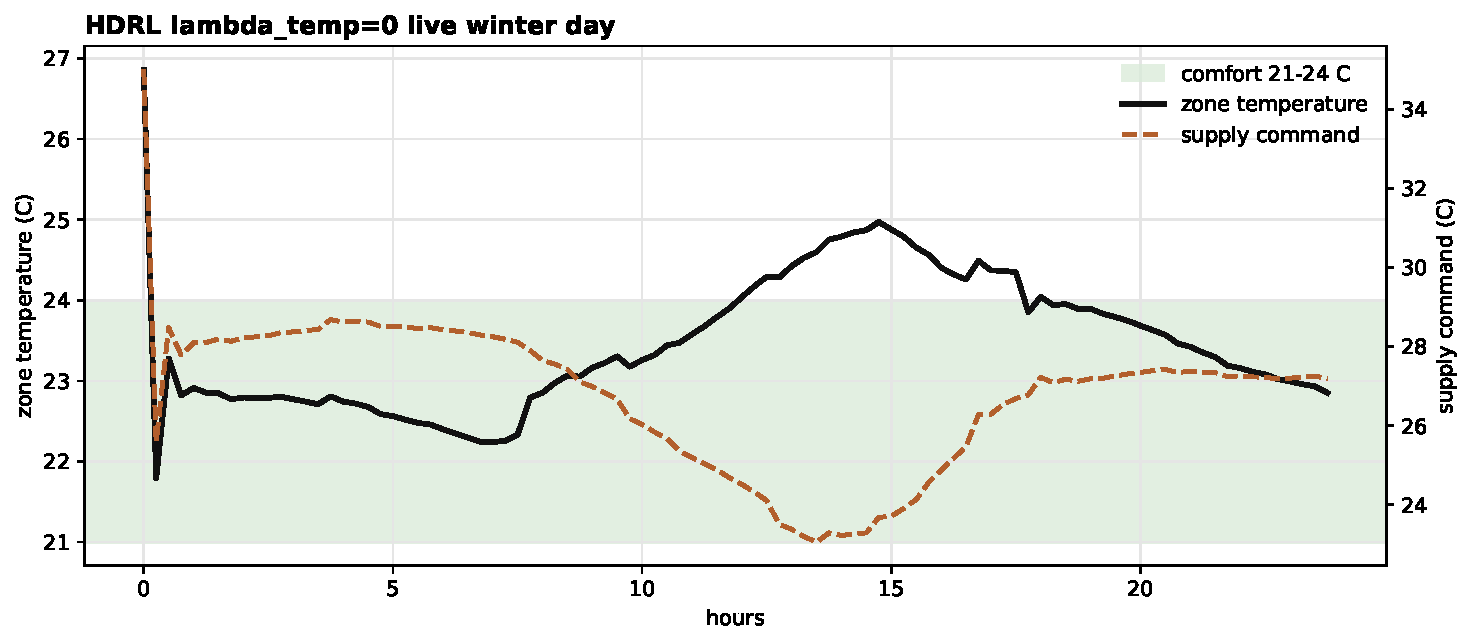
\includegraphics[width=0.88\linewidth]{block2_hdrl_l000_winter_tracking.pdf}
  \caption{Representative HDRL $\lambda_T=0$ winter tracking trace. The trace provides the physical reading behind the sweep table.}
  \label{fig:hdrl_trace}
\end{figure}

\section{MORL observation ablation: 5D failure to 17D success}

MORL initially failed with a 5D observation interface consisting of zone temperature, ambient temperature, hour, day, and occupancy. With the same hybrid backend, the 5D policy obtained RMSE$_T=4.96\,^\circ$C, violation $74.5\%$, and $m_s=1.046$. Replacing the observation with the 17D TSup-style vector recovers a usable policy: RMSE$_T=0.72\,^\circ$C, violation $4.9\%$, and $m_s=0.099$. Thus the dominant MORL bottleneck was not the reward scalarization alone; it was the observation geometry through which the policy inferred actuator-relevant state.

\begin{table}[t]
\centering
\caption{MORL observation-interface ablation. The backend is hybrid in both cases; the observation interface changes from 5D to 17D.}
\label{tab:morl5d17d}
\small
\begin{tabular}{lrrrrr}
\toprule
Variant & RMSE$_T$ ($^\circ$C) & MAE$_T$ ($^\circ$C) & Within 1$^\circ$C (\%) & Violation (\%) & $m_s$ \\
\midrule
MORL 5D basic & 4.96 & 4.17 & 19 & 74.5 & 1.046 \\
MORL 17D power-only & 0.72 & 0.56 & 83 & 4.9 & 0.099 \\
\bottomrule
\end{tabular}
\end{table}

\begin{figure}[t]
  \centering
  
\includegraphics[width=0.84\linewidth]{final17_fig09_morl_5d_failure_17d_success.pdf}
  \caption{MORL 5D failure and 17D recovery. The observation interface, not only the scalarized reward, determines whether MORL is viable.}
  \label{fig:morl5d17d}
\end{figure}

\section{MORL Pareto front and seed variance}

The MORL Pareto sweep varies comfort and energy weights while keeping safety weight at zero. Energy-only control collapses comfort ($m_s=1.588$, violation $86.8\%$). Comfort-heavy settings are much more stable: the 100/0 point gives $m_s=0.032$ at seed 42, while the legacy 80/20 point gives $m_s=0.099$. The 75/25 practical canonical has lower mean $m_s$ than the 50/50 neutral canonical, but both remain seed-sensitive when expanded to $N=5$.

\begin{table}[t]
\centering
\caption{MORL Pareto and N=5 canonical seed analysis. Single-seed Pareto points are shown separately from the N=5 canonical extensions.}
\label{tab:morl_pareto_seed}
\small
\begin{tabular}{lrrrr}
\toprule
Preference / statistic & RMSE$_T$ ($^\circ$C) & Violation (\%) & $m_s$ & Interpretation \\
\midrule
0/100 seed 42 & 8.359 & 86.76 & 1.588 & energy-only collapse \\
25/75 seed 42 & 0.912 & 11.39 & 0.173 & energy-weighted usable \\
50/50 N=5 mean $\pm$ std & 0.893 $\pm$ 0.081 & 13.01 $\pm$ 6.62 & 0.187 $\pm$ 0.078 & high variance \\
75/25 N=5 mean $\pm$ std & 0.799 $\pm$ 0.100 & 9.23 $\pm$ 6.67 & 0.139 $\pm$ 0.085 & lower mean, higher CV \\
80/20 seed 42 & 0.725 & 4.87 & 0.099 & legacy canonical \\
100/0 seed 42 & 0.631 & 1.49 & 0.032 & best seed-42 comfort \\
\bottomrule
\end{tabular}
\end{table}

\begin{figure}[t]
  \centering
  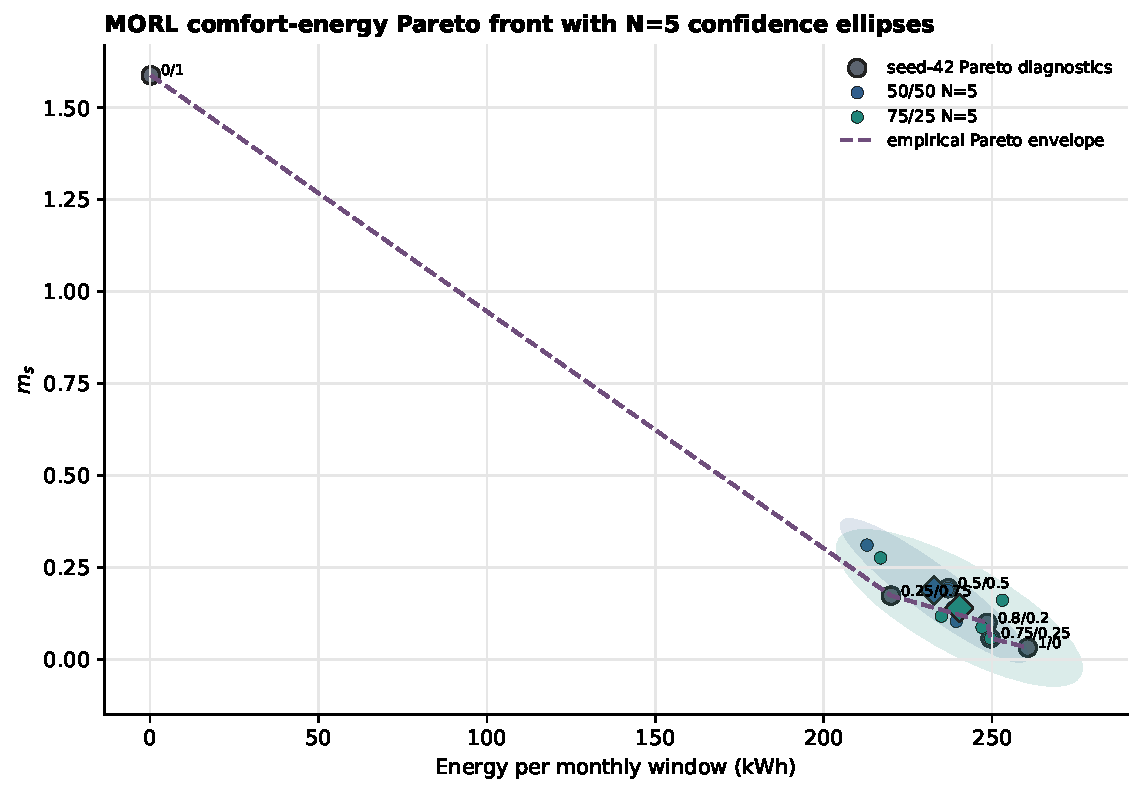
\includegraphics[width=0.86\linewidth]{block2_q1_polish_morl_pareto_ellipses.pdf}
  \caption{MORL comfort--energy Pareto front with N=5 confidence ellipses for
  the two canonical points. The dashed envelope connects empirically
  non-dominated seed-42 diagnostics; the ellipses show seed covariance in
  energy--\(m_s\) space.}
  \label{fig:morl_pareto}
\end{figure}

The N=5 seed extension is the most important MORL audit result. The neutral 50/50 canonical has $m_s=0.187\pm0.078$ (CV $0.418$), and the practical 75/25 canonical has $m_s=0.139\pm0.085$ (CV $0.613$). Seed 46 is an outlier in both groups. Because the replay determinism audit produced bit-identical BOPTEST trajectories for the same policy, this variance is attributed to PPO/ERAM training stochasticity rather than simulator noise.

\section{Seasonal variance falsification}

At $N=3$, the practical canonical appeared to show near-deterministic winter behavior and a seasonal inversion relative to the neutral canonical. That pattern motivated a pre-registered falsification test before seeds 45 and 46 were trained. The direction-specific predictions were: February winter $\sigma(m_s)<0.005$, June summer $\sigma(m_s)>0.05$, and winter neutral/practical variance ratio greater than 20. At $N=5$, the central predictions failed. February practical $\sigma(m_s)$ increased to approximately $0.168$--$0.188$ depending on the exact monthly table, and the neutral/practical winter variance ratio collapsed to order one rather than 20.

\begin{figure}[t]
  \centering
  
\includegraphics[width=0.88\linewidth]{block2_morl_17d_seasonal_heatmap.pdf}
  \caption{MORL seasonal performance heatmap under the 17D interface. The figure shows monthly structure but does not support the earlier N=3 mechanism claim after N=5 extension.}
  \label{fig:morl_heatmap}
\end{figure}

\begin{figure}[t]
  \centering
  
\includegraphics[width=0.88\linewidth]{block2_morl_seasonal_variance_inversion.pdf}
  \caption{Post-N=5 seasonal variance diagnostic. The earlier seasonal-inversion hypothesis is reported as falsified, not retained as a positive mechanism claim.}
  \label{fig:seasonal_falsification}
\end{figure}

This is a scientific success of the pre-registration protocol rather than a failure of the project. The honest conclusion is narrower and stronger: MORL remains promising in mean performance, especially at comfort-leaning preferences, but it is not deployment-stable without explicit stabilization such as validation-based checkpoint selection, early stopping, or ensemble policy selection. Those stabilization methods are future work because the Block 2 canonical protocol is fixed to final-epoch policy evaluation.

\section{Results II conclusion}

Block 2 establishes four controller-side claims.

First, predictive fidelity and RL training utility are not equivalent. Direct v3.5 is more accurate as a digital twin but fails as a rollout environment, producing live BOPTEST comfort violations above 77\%. Second, role separation works: v3 should provide smooth rollout dynamics, while v3.5 should act as a frozen physical censor through disagreement reward shaping. This produces the canonical hybrid result with $m_s=0.087$ on peak and $m_s=0.041$ on typical windows. Third, controller families respond differently to the same regularizer. HDRL rejects the thermostatic $\lambda_T=0.10$ setting and performs best at $\lambda_T=0$. Fourth, MORL is viable only after the observation interface is expanded to 17D, but its N=5 canonical analysis reveals high seed variance and falsifies the earlier N=3 seasonal-inversion mechanism.

The engineering implication is that hybrid surrogate RL is not a single architecture choice. It is a role-allocation problem: rollout smoothness, physical censoring, observation geometry, controller family, and seed stabilization must be treated as separate design axes. This conclusion is the bridge to Block 3, where the fixed bestest-air controller recipe is transferred to hydronic-family BOPTEST testcases.

\end{document}
